
    \begin{itemize}
        \item Classification lies at the heart of both human and machine intelligence. 
        \item Deciding what letter, word, or image has been presented to our senses, recognizing faces or voices, sorting mail, assigning grades to homeworks.
        \item These are all examples of assigning a category to an input.
        \item The goal of classification is to take a single observation, extract some useful features, and thereby classify the observation into one of a set of discrete classes.
        \item  Most cases of classification in language processing are done via supervised machine learning. 
        \item This slides are based on the course material by Daniel Jurafsky : \url{https://web.stanford.edu/~jurafsky/slp3/4.pdf} 
    \end{itemize}   

Example 1: Spam Classification

\begin{figure}[h]
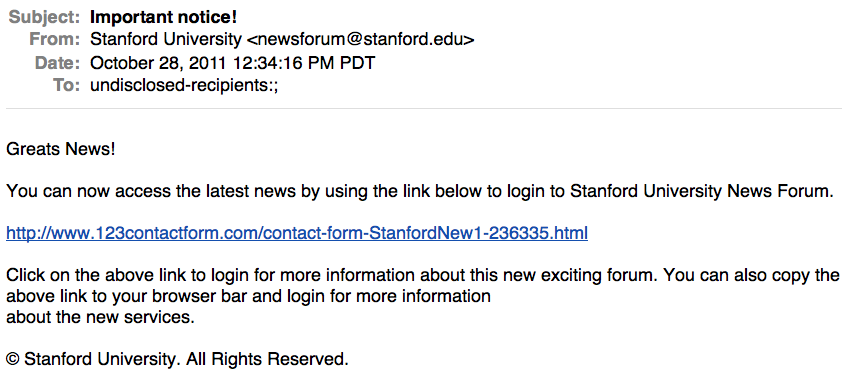
\includegraphics[scale = 0.35]{pics/spam.png}
\end{figure}


Example 2: Who wrote which Federalist papers?

    \begin{itemize}
        \item 1787-8: Anonymous essays attempted to convince New York to ratify the U.S Constitution: Jay, Madison, Hamilton.
        \item Authorship of 12 of the letters is in dispute.
        \item 1963: Solved by Mosteller and Wallace using Bayesian methods.
    \end{itemize}

    \begin{center}
        \begin{figure}[h]
            \begin{minipage}{0.3\textwidth}
                \centering
                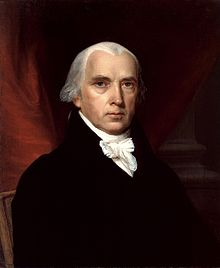
\includegraphics[width=\linewidth]{pics/madison.png}
                \caption{James Madison}
            \end{minipage}\hfill
            \begin{minipage}{0.3\textwidth}
                \centering
                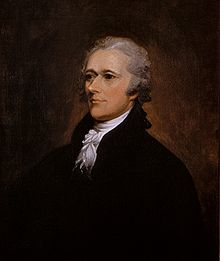
\includegraphics[width=\linewidth]{pics/hamilton.png}
                \caption{Alexander Hamilton}
            \end{minipage}
        \end{figure}
    \end{center}


Example 3: What is the subject of this medical article?

\begin{figure}[h]
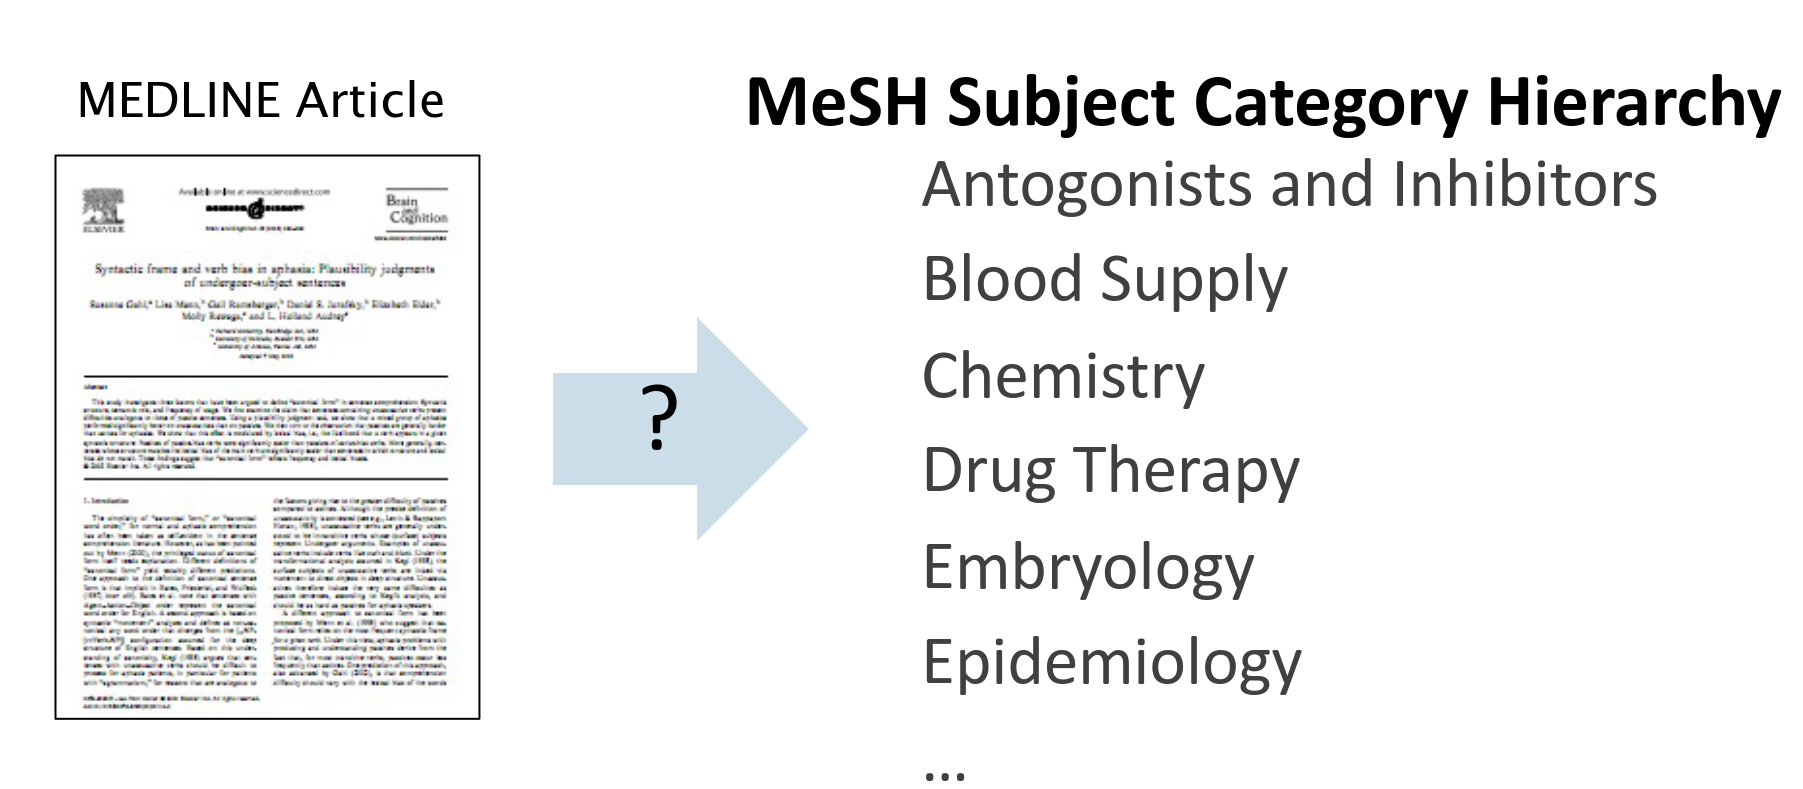
\includegraphics[scale = 0.2]{pics/medarticle.png}
\end{figure}



Example 4: Positive or negative movie review?
    \begin{itemize}
     \item  \textcolor{blue}{\textbf{+}}   ...zany characters and \textcolor{blue}{richly} applied satire, and some \textcolor{blue}{great} plot twists 
     \item   \textcolor{red}{\textbf{-}} It was \textcolor{red}{pathetic}. The \textcolor{red}{worst} part about it was the boxing scenes... 
    \item   \textcolor{blue}{\textbf{+}}  ...\textcolor{blue}{awesome} caramel sauce and sweet toasty almonds. I \textcolor{blue}{love} this place! \\
     \item \textcolor{red}{\textbf{-}} ...\textcolor{red}{awful} pizza and \textcolor{red}{ridiculously} overpriced... 
    \end{itemize}



\paragraph{Why sentiment analysis?}
    \begin{itemize}
        \item Movie: Is this review positive or negative?
        \item Products: What do people think about the new iPhone?
        \item Public sentiment: How is consumer confidence?
        \item Politics: What do people think about this candidate or issue?
        \item Prediction: Predict election outcomes or market trends from sentiment.
    \end{itemize}


\paragraph{Basic Sentiment Classification}
    Sentiment analysis is the detection of attitudes.
    \begin{itemize}
        \item Simple task we focus on in this class
        \begin{itemize}
            \item Is the attitude of this text positive or negative?
        \end{itemize}
    \end{itemize}



\paragraph{Summary: Text Classification}
    Text classification can be applied to various tasks, including:
    \begin{itemize}
        \item Sentiment analysis
        \item Spam detection
        \item Authorship identification
        \item Language identification
        \item Assigning subject categories, topics, or genres
        \item ...
    \end{itemize}


\section{Text Classification: Definition}
    \textbf{Input}:
    \begin{itemize}
        \item A document $d$
        \item A fixed set of classes $C = \{c_1, c_2, \ldots, c_J\}$
    \end{itemize}
    
    \textbf{Output}: A predicted class $c \in C$


\subsection{Classification Methods: Hand-coded rules}
    Rules based on combinations of words or other features
    \begin{itemize}
        \item Spam: \textit{black-list-address} OR (\textit{“dollars” AND “you have been selected”})
        \item Accuracy can be high if rules carefully refined by experts
        \item But building and maintaining these rules is expensive
    \end{itemize}

\subsection{Classification Methods: Supervised Machine Learning}
    \textbf{Input}:
    \begin{itemize}
        \item A document $d$
        \item A fixed set of classes $C = \{c_1, c_2, \ldots, c_J\}$
        \item A training set of $m$ hand-labeled documents: $(d_1, c_1), (d_2, c_2), \ldots, (d_m, c_m)$
    \end{itemize}
    
    \textbf{Output}:
    \begin{itemize}
        \item A learned classifier $\gamma: d \to c$
    \end{itemize}

    Any kind of classifier can be used:
    \begin{itemize}
        \item Naïve Bayes
        \item Logistic regression
        \item Neural networks
        \item k-Nearest Neighbors
        % Add more classifiers as needed
    \end{itemize}

 \subsection{Supervised Learning Problems}
  \begin{itemize}
    \item We have training examples $x^{(i)}$, $y^{(i)}$ for $i = 1, \ldots, m$. Each $x^{(i)}$ is an input, each $y^{(i)}$ is a label.
    \item Task is to learn a function $f$ mapping inputs $x$ to labels $f(x)$.
    \item Conditional models:
    \begin{itemize}
      \item Learn a distribution $p(y|x)$ from training examples.
      \item For any test input $x$, define $f(x) = \arg \max_y p(y|x)$.
    \end{itemize}
  \end{itemize}

  \subsection{Generative Models}
  \begin{itemize}
    \item Given training examples $x^{(i)}$, $y^{(i)}$ for $i = 1, \ldots, m$. The task is to learn a function $f$ that maps inputs $x$ to labels $f(x)$.
    \item Generative models:
    \begin{itemize}
      \item Learn the joint distribution $p(x, y)$ from the training examples.
      \item Often, we have $p(x, y) = p(y)p(x|y)$.
      \item Note: We then have
      \[
        p(y|x) = \frac{p(y)p(x|y)}{p(x)} \quad \text{where} \quad p(x) = \sum_y p(y)p(x|y).
      \]
    \end{itemize}
  \end{itemize}


\subsection{Classification with Generative Models}
  \begin{itemize}
    \item Given training examples $x^{(i)}$, $y^{(i)}$ for $i = 1, \ldots, m$. The task is to learn a function $f$ that maps inputs $x$ to labels $f(x)$.
    \item Generative models:
    \begin{itemize}
      \item Learn the joint distribution $p(x, y)$ from the training examples.
      \item Often, we have $p(x, y) = p(y)p(x|y)$.
    \end{itemize}
    \item Output from the model:
\[
\begin{aligned}
f(x) = \arg\max_y p(y|x) &= \arg\max_y \frac{p(y)p(x|y)}{p(x)} \\
&= \arg\max_y p(y)p(x|y)
\end{aligned}
\]
  \end{itemize}



\section{Naive Bayes Intuition}
    Naive Bayes is a simple ("naive") classification method based on Bayes' rule.
    \begin{itemize}
        \item Relies on a very simple representation of a document: \textit{Bag of words}
    \end{itemize}


\paragraph{The Bag of Words Representation}

\begin{figure}[h]
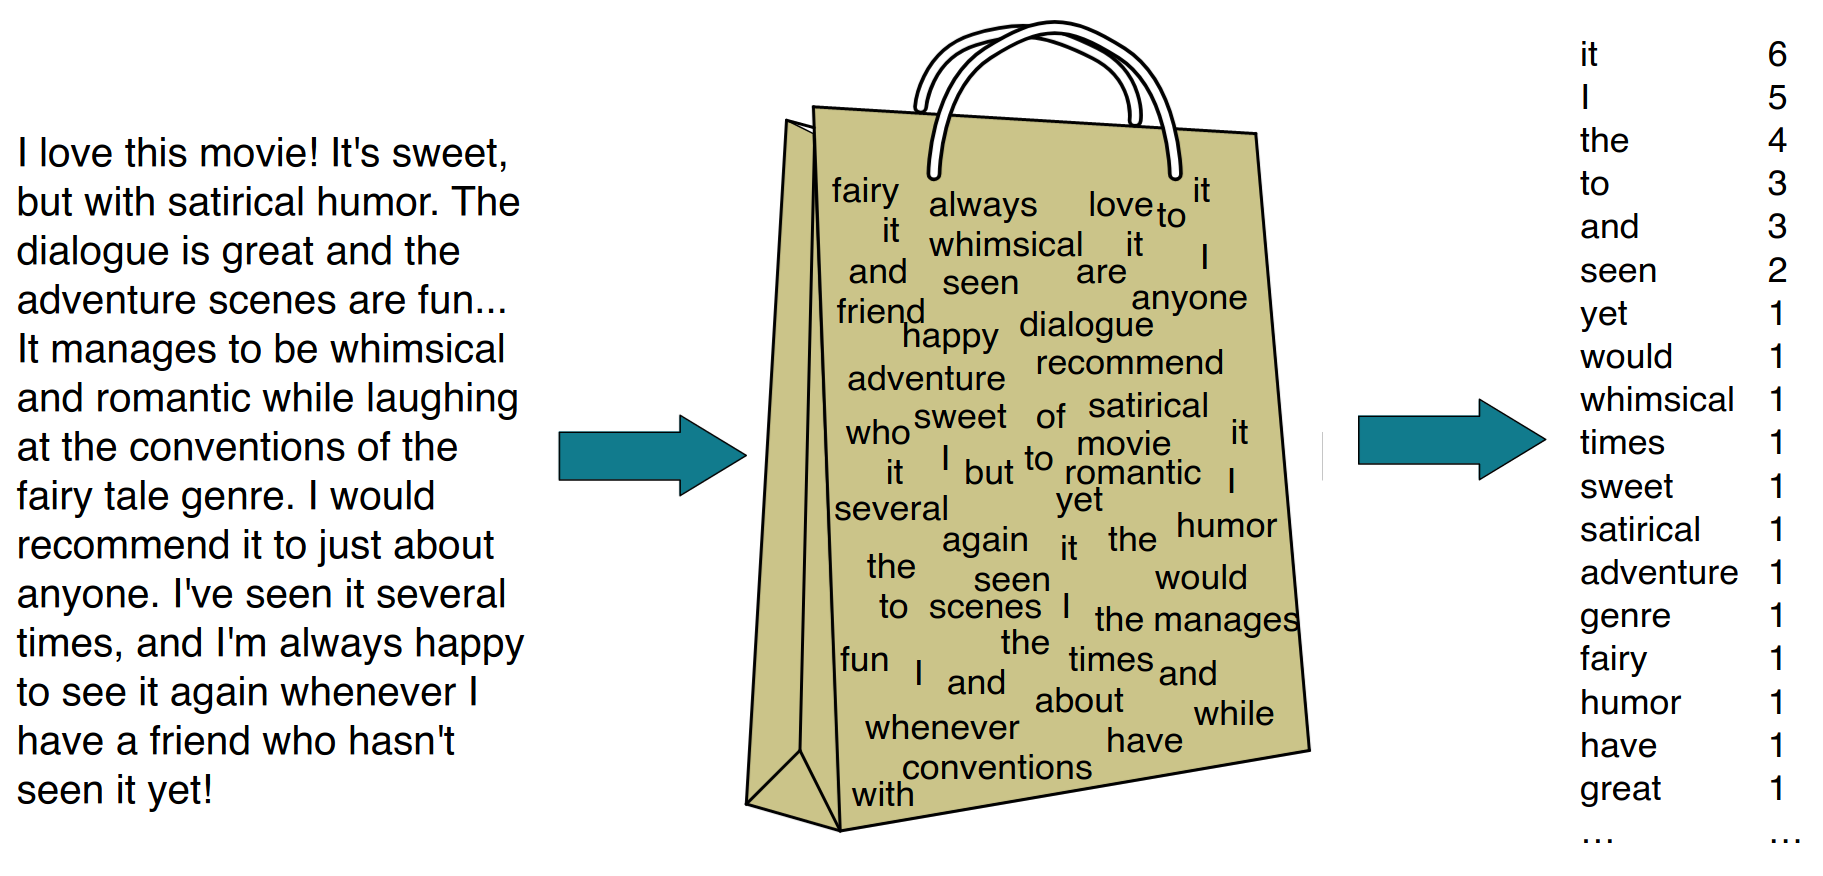
\includegraphics[scale = 0.22]{pics/bow.png}
\end{figure}


\subsection{Bayes' Rule Applied to Documents and Classes}
    For a document $d$ and a class $c$:
    \[
    P(c | d) = \frac{P(d | c)P(c)}{P(d)}
    \]


\section{Naive Bayes Classifier}
\begin{itemize}
    \item MAP stands for "maximum a posteriori," which represents the most likely class:
    \[
    c_{\text{MAP}} = \arg\max_{c \in C} P(c | d)
    \]
    \item To calculate the most likely class, we apply Bayes' rule:
    \[
    = \arg\max_{c \in C} \frac{P(d | c)P(c)}{P(d)}
    \]
    \item Finally, we can drop the denominator since it remains constant for all classes:
    \[
    = \arg\max_{c \in C} P(d | c)P(c)
    \]
    \item To classify document $d$, we use the MAP estimate:
    \[
    c_{\text{MAP}} = \arg\max_{c \in C} P(d | c)P(c)
    \]
    \item The document $d$ is represented as a set of features $x_1, x_2, \ldots, x_n$.
    \item The classifier calculates the conditional probability of the features given a class and the prior probability of the class:
    \[
    = \arg\max_{c \in C} P(x_1, x_2, \ldots, x_n | c)P(c)
    \]
    \item The term $P(x_1, x_2, \ldots, x_n | c)$ represents the "likelihood" of the features given the class.
    \item The term $P(c)$ represents the "prior" probability of the class.
    \item The Naïve Bayes classifier \cite{mccallum1998comparison} calculates the MAP estimate by considering the likelihood and prior probabilities:
    \[
    c_{\text{MAP}} = \arg\max_{c \in C} P(x_1, x_2, \ldots, x_n | c)P(c)
    \]
    \item The probability of the features given the class, $P(x_1, x_2, \ldots, x_n | c)$, can be estimated by counting the relative frequencies in a corpus.
    \item The prior probability of the class, $P(c)$, represents how often this class occurs.
    \item Without some simplifying assumptions, estimating the probability of every possible combination of
features in $P(x_1, x_2, \ldots, x_n | c)$ would require huge numbers of parameters and impossibly large training sets. 
\item Naive Bayes classifiers therefore make two simplifying assumptions.
\end{itemize}


\subsection{Multinomial Naive Bayes Independence Assumptions}

\begin{itemize}
    \item Bag of Words assumption: We assume that the position of words in the document does not matter.
    \item Conditional Independence assumption: We assume that the feature probabilities $P(x_i | c_j)$ are independent given the class $c_j$.
    \item In the Multinomial Naive Bayes classifier, the probability of a document with features $x_1, x_2, \ldots, x_n$ given class $c$ can be calculated as:
    \[
    P(x_1, x_2, \ldots, x_n | c) = P(x_1 | c) \cdot P(x_2 | c) \cdot P(x_3 | c) \cdot \ldots \cdot P(x_n | c)
    \]
\end{itemize}

\subsection{Multinomial Naive Bayes Classifier}
\begin{itemize}
    \item The Maximum A Posteriori (MAP) estimate for class $c$ in the Multinomial Naive Bayes classifier is given by:
    \[
    c_{\text{MAP}} = \arg\max_{c \in C} P(x_1, x_2, \ldots, x_n | c)P(c)
    \]
    \item Alternatively, we can write it as:
    \[
    c_{\text{NB}} = \arg\max_{c \in C} P(c_j) \prod_{x \in X} P(x | c)
    \]
    \item $P(c_j)$ represents the prior probability of class $c_j$.
    \item $\prod_{x \in X} P(x | c)$ represents the likelihood of the features $x_1, x_2, \ldots, x_n$ given class $c$.
\end{itemize}


\subsection{Applying Multinomial Naive Bayes Classifiers to Text Classification}
\begin{itemize}
    \item The Multinomial Naive Bayes classifier for text classification can be applied as follows:
    \[
    c_{\text{NB}} = \arg\max_{c_j \in C} P(c_j) \prod_{i \in \text{positions}} P(x_i | c_j)
    \]
    \item $c_{\text{NB}}$ represents the predicted class for the test document.
    \item $C$ is the set of all possible classes.
    \item $P(c_j)$ is the prior probability of class $c_j$.
    \item $\prod_{i \in \text{positions}} P(x_i | c_j)$ calculates the likelihood of each feature $x_i$ at position $i$ given class $c_j$.
    \item The product is taken over all word positions in the test document.
\end{itemize}


\subsection{Problems with Multiplying Lots of Probabilities}
\begin{itemize}
    \item Multiplying lots of probabilities can result in floating-point underflow, especially when dealing with small probabilities.
    \item Example: $0.0006 \times 0.0007 \times 0.0009 \times 0.01 \times 0.5 \times 0.000008 \ldots$
    \item Idea: Use logarithms, as $\log(ab) = \log(a) + \log(b)$.
    \item Instead of multiplying probabilities, we can sum the logarithms of probabilities.
    \item The Multinomial Naive Bayes classifier can be expressed using logarithms as follows:
    \[
    c_{\text{NB}} = \arg\max_{c_j \in C} \left(\log(P(c_j)) + \sum_{i \in \text{position}} \log(P(x_i | c_j))\right)
    \]
    \item By taking logarithms, we avoid the issue of floating-point underflow and perform calculations in the log space.
     \item The classifier becomes a linear model, where the prediction is the argmax of a sum of weights (log probabilities) and the inputs (log conditional probabilities):
    \item Thus, Naïve Bayes is a linear classifier, operating in the log space.
    
    
\end{itemize}

\subsection{Learning the Multinomial Naive Bayes Model}
First attempt: Maximum Likelihood Estimates
\begin{itemize}
    \item The probabilities are estimated using the observed counts in the training data.
    \item The prior probability of a class $c_j$ is estimated as:
    \[
    \hat{P}(c_j) = \frac{N_{c_j}}{N_{\text{total}}}
    \]
    where $N_{c_j}$ is the number of documents in class $c_j$ and $N_{\text{total}}$ is the total number of documents.
    \item The estimate of the probability of word $w_i$ given class $c_j$ is calculated as:
    \[
    \hat{P}(w_i | c_j) = \frac{{\text{{count}}(w_i, c_j)}}{\sum_{w\in V}{\text{{count}}(w, c_j)}}
    \]
    where $w \in V$ represents a word in the vocabulary $V$.
    \item The denominator is the sum of counts of all words in the vocabulary within class $c_j$.
\end{itemize}


\subsection{Parameter Estimation}

To estimate the parameters of the Multinomial Naive Bayes model, we follow these steps:

\begin{itemize}
  \item Create a mega-document for each topic $c_j$ by concatenating all the documents in that topic.
  \item We calculate the frequency of word $w_i$ in the mega-document, which represents the fraction of times word $w_i$ appears among all words in the documents of topic $c_j$.
  \item The estimated probability $\hat{P}(w_i | c_j)$ of word $w_i$ given class $c_j$ is obtained by dividing the count of occurrences of $w_i$ in the mega-document of topic $c_j$ by the total count of words in the mega-document:
  \[
  \hat{P}(w_i | c_j) = \frac{{\text{{count}}(w_i, c_j)}}{\sum_{w\in V}{\text{{count}}(w, c_j)}}
  \]
  Here, $\text{{count}}(w_i, c_j)$ represents the number of times word $w_i$ appears in the mega-document of topic $c_j$, and $\text{{count}}(w, c_j)$ is the total count of words in the mega-document.
\end{itemize}


\subsection{Zero Probabilities and the Issue of Unseen Words}
\begin{itemize}
    \item Consider the scenario where we have not encountered the word ``fantastic'' in any training documents classified as positive (thumbs-up).
    \item Using maximum likelihood estimation, the probability $\hat{P}(\text{``fantastic''} \mid \text{positive})$ would be calculated as:
    \[
    \hat{P}(\text{``fantastic''} \mid \text{positive}) = \frac{\text{count}(\text{``fantastic''}, \text{positive})}{\sum_{w \in V} \text{count}(w, \text{positive})}
    \]
    \item In this case, the count of the word ``fantastic'' in positive documents is zero, leading to a zero probability:
    \[
    \hat{P}(\text{``fantastic''} \mid \text{positive}) = \frac{0}{\sum_{w \in V} \text{count}(w, \text{positive})} = 0
    \]
    \item However, zero probabilities cannot be conditioned away, regardless of the other evidence present.
    \item This poses a problem when calculating the maximum a posteriori (MAP) estimate, which is used for classification:
    \[
    c_{\text{MAP}} = \arg\max_c \left(\hat{P}(c) \prod_{i} \hat{P}(x_i \mid c)\right)
    \]
    \item With a zero probability for a word, the entire expression becomes zero, regardless of other evidence.
\end{itemize}




\subsection{Laplace (Add-1) Smoothing for Naïve Bayes}
Handling zero probabilities with Laplace (Add-1) smoothing
\begin{itemize}
    \item To address the problem of zero probabilities, we can employ Laplace (Add-1) smoothing technique.
    \item The smoothed estimate $\hat{P}(w_i \mid c)$ is calculated as:
    \[
    \hat{P}(w_i \mid c) = \frac{\text{count}(w_i, c) + 1}{\sum_{w \in V} (\text{count}(w, c) + 1)}
    \]
    \item Here, an additional count of 1 is added to both the numerator and the denominator.
    \item The denominator is adjusted by adding the size of the vocabulary $V$ to ensure proper normalization.
    \item By doing so, we prevent zero probabilities and allow some probability mass to be distributed to unseen words.
    \item This smoothing technique helps to mitigate the issue of unseen words and avoids the complete elimination of certain classes during classification.
\end{itemize}






\subsection{Multinomial Naïve Bayes: Learning}
Learning the Multinomial Naïve Bayes Model
\begin{itemize}
    \item In order to learn the parameters of the model, we need to calculate the terms $P(c_j)$ and $P(w_k \mid c_j)$.
    \item For each class $c_j$ in the set of classes $C$, we perform the following steps:
    \begin{itemize}
        \item Retrieve all the documents $docs_j$ that belong to class $c_j$.
        \item Calculate the term $P(w_k \mid c_j)$ for each word $w_k$ in the vocabulary $V$:
        \[
        P(w_k \mid c_j) = \frac{{n_k + \alpha}}{{n + \alpha \cdot \lvert \text{Vocabulary} \rvert}}
        \]
        where $n_k$ represents the number of occurrences of word $w_k$ in the concatenated document $Text_j$.
        \item Calculate the prior probability $P(c_j)$:
        \[
        P(c_j) = \frac{{\lvert docs_j \rvert}}{{\lvert \text{total number of documents} \rvert}}
        \]
    \end{itemize}
    \item To calculate $P(w_k \mid c_j)$, we need to extract the vocabulary $V$ from the training corpus.
\end{itemize}


\subsection{Unknown Words}
Dealing with unknown words in the test data:
\begin{itemize}
    \item When we encounter unknown words in the test data that do not appear in the training data or vocabulary, we ignore them.
    \item We remove these unknown words from the test document as if they were not present at all.
    \item We do not assign any probability to these unknown words in the classification process.
\end{itemize}

Why don't we build an unknown word model?
\begin{itemize}
    \item Building a separate model for unknown words is not generally helpful.
    \item Knowing which class has more unknown words does not provide useful information for classification.
\end{itemize}

\subsection{Stop Words}

Stop words are frequently used words like "the" and "a" that are often considered to have little or no significance in text classification. Some systems choose to ignore stop words in the classification process. Here is how it is typically done:

\begin{itemize}
    \item Sort the vocabulary by word frequency in the training set.
    \item Create a stopword list by selecting the top 10 or 50 most frequent words.
    \item Remove all stop words from both the training and test sets, treating them as if they were never there.
\end{itemize}

However, removing stop words doesn't usually improve the performance of Naive Bayes classifiers. Therefore, in practice, most Naive Bayes algorithms use all words and do not utilize stopword lists.


\section{Worked Sentiment Example}

\textbf{Training data:} 

\begin{table}[h]
\centering
\begin{tabular}{|c|p{0.7\textwidth}|}
\hline
\textbf{Category} & \textbf{Text} \\
\hline
Negative & Just plain boring, entirely predictable and lacks energy. \\
\hline
Negative & No surprises and very few laughs. \\
\hline
Positive & Very powerful. \\
\hline
Positive & The most fun film of the summer. \\
\hline
\end{tabular}
\end{table}


\textbf{Test:} 
\begin{table}[h]
\centering
\begin{tabular}{|c|p{0.7\textwidth}|}
\hline
\textbf{Category} & \textbf{Text} \\
\hline
? & Predictable with no fun. \\
\hline
\end{tabular}
\end{table}

\begin{figure}[h]
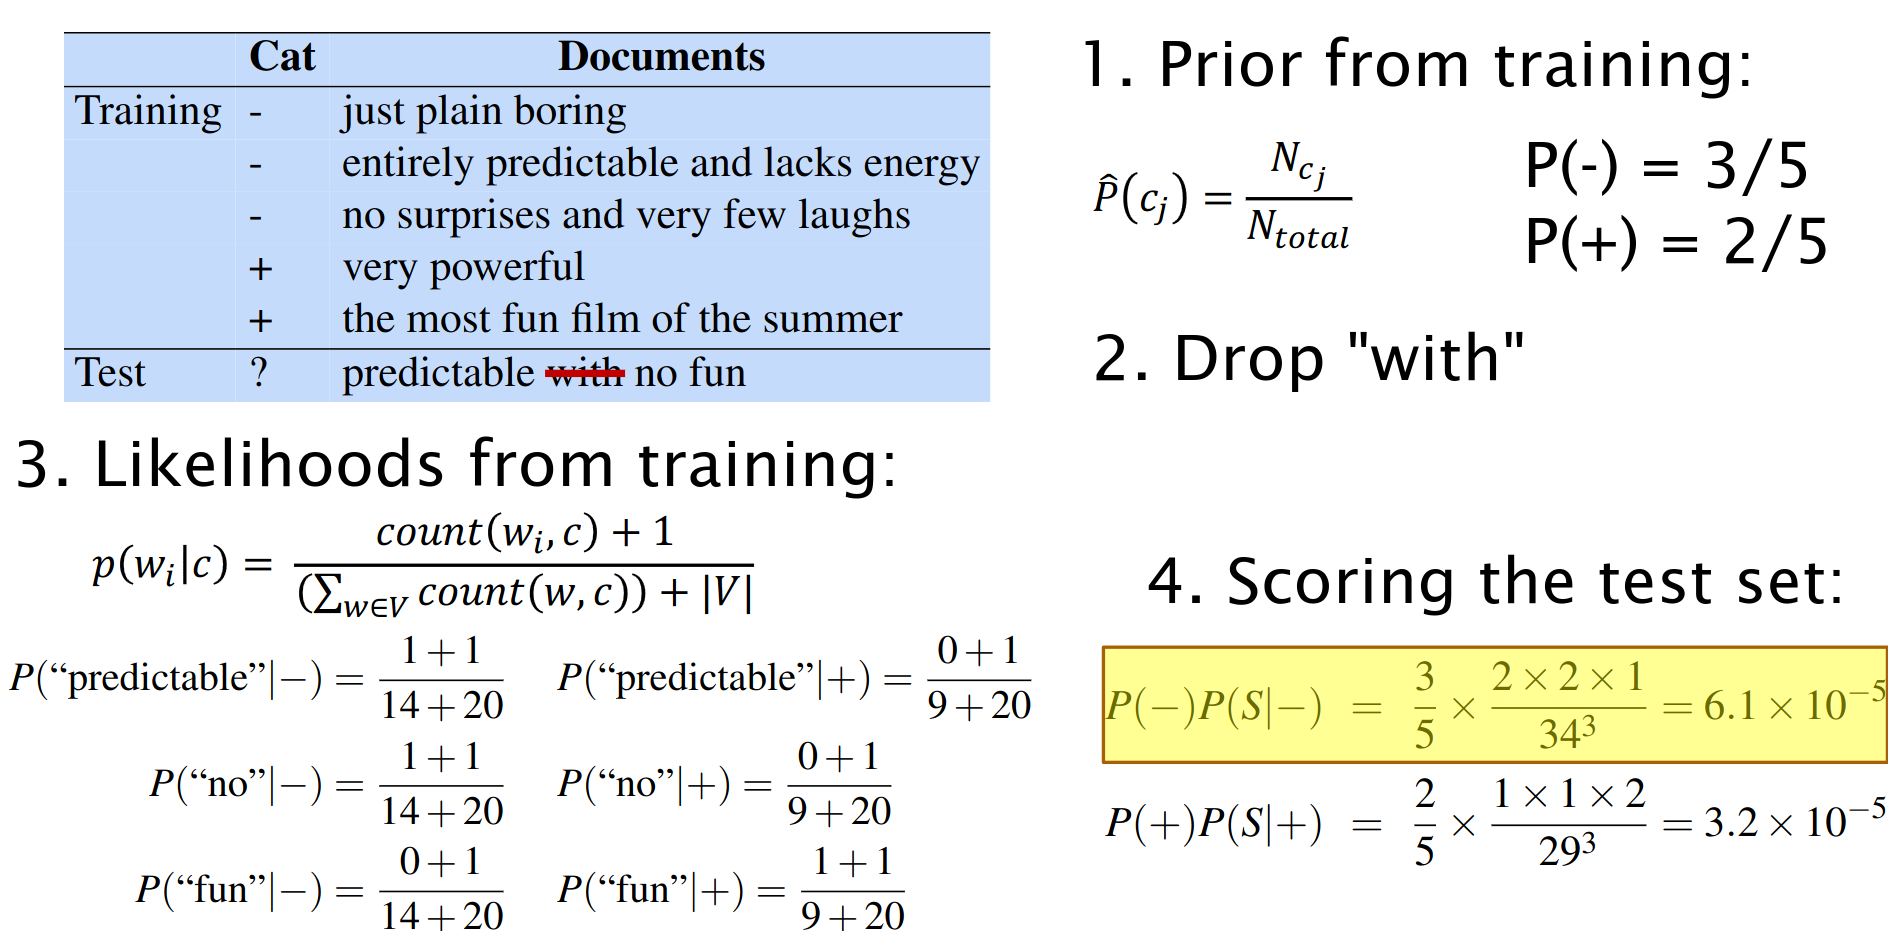
\includegraphics[scale = 0.23]{pics/naive_example.png}
\end{figure}


\section{Naive Bayes as a Language Model}

\begin{itemize}
 \item When using individual word features and considering all words in the text, naive Bayes has an important similarity to language modeling. 
 \item Specifically, a naive Bayes model can be viewed as a set of class-specific unigram language models, in which the model for each class instantiates a unigram language model.
 \item The likelihood features from the naive Bayes model assign a probability to each word $P(word|c)$, and the model also assigns a probability to each sentence:
\[P(s|c) = \prod_{i\in positions} P(w_i|c)\]
\end{itemize}
Consider a naive Bayes model with the classes positive (+) and negative (-) and the following model parameters:
\begin{center}
\begin{tabular}{ccc}
\textbf{w} & $P(w|+)$ & $P(w|-)$ \\
I & 0.1 & 0.2 \\
love & 0.1 & 0.001 \\
this & 0.01 & 0.01 \\
fun & 0.05 & 0.005 \\
film & 0.1 & 0.1 \\
... & ... & ...
\end{tabular}
\end{center}



\begin{itemize}
 \item  Each of the two columns above instantiates a language model that can assign a probability to the sentence "I love this fun film":
\[P("\text{I love this fun film}"|+) = 0.1 \times 0.1 \times 0.01 \times 0.05 \times 0.1 = 0.0000005\]
\[P("\text{I love this fun film}"|-) = 0.2 \times 0.001 \times 0.01 \times 0.005 \times 0.1 = 0.0000000010\]

\item As it happens, the positive model assigns a higher probability to the sentence:
\[P(s|pos) > P(s|neg)\]

\item Note that this is just the likelihood part of the naive Bayes model; once we multiply in the prior, a full naive Bayes model might well make a different classification decision.
\end{itemize}




\section{Evaluation}

\begin{itemize}
 \item Let's consider just binary text classification tasks. 
 \item Imagine you're the CEO of Delicious Pie Company. 
\item You want to know what people are saying about your pies. 
\item So you build a "Delicious Pie" tweet detector with the following classes:
\begin{itemize}
\item Positive class: tweets about Delicious Pie Co
\item Negative class: all other tweets
\end{itemize}
\end{itemize}



\subsection{The 2-by-2 Confusion Matrix}
\begin{table}[h]
\centering
\begin{tabular}{|c|c|c|}
\hline
\textbf{} & \textbf{System Positive} & \textbf{System Negative} \\
\hline
\textbf{Gold Positive} & True Positive (TP) & False Negative (FN) \\
\hline
\textbf{Gold Negative} & False Positive (FP) & True Negative (TN) \\
\hline
\end{tabular}
\end{table}

\textbf{Recall} (also known as \textbf{Sensitivity} or \textbf{True Positive Rate}):
\[ \text{Recall} = \frac{TP}{TP + FN} \]

\textbf{Precision}:
\[ \text{Precision} = \frac{TP}{TP + FP} \]

\textbf{Accuracy}:
\[ \text{Accuracy} = \frac{TP + TN}{TP + FP + TN + FN} \]


\subsection{Evaluation: Accuracy}
Why don't we use accuracy as our metric?

Imagine we saw 1 million tweets:
\begin{itemize}
\item 100 of them talked about Delicious Pie Co.
\item 999,900 talked about something else.
\end{itemize}

We could build a dumb classifier that just labels every tweet "not about pie":
\begin{itemize}
\item It would get 99.99\% accuracy!!! Wow!!!!
\item But it would be useless! It doesn't return the comments we are looking for!
\end{itemize}

That's why we use precision and recall instead.

\subsection{Evaluation: Precision and Recall}
\textbf{Precision} measures the percentage of items the system detected (i.e., items the system labeled as positive) that are in fact positive (according to the human gold labels).

\[
\text{Precision} = \frac{\text{True Positives}}{\text{True Positives + False Positives}}
\]


\textbf{Recall} measures the percentage of items that were correctly identified by the system out of all the items that should have been identified.

\[
\text{Recall} = \frac{\text{True Positives}}{\text{True Positives + False Negatives}}
\]



\subsection{Why Precision and Recall?}
Consider our dumb pie-classifier that just labels nothing as "about pie."

\begin{itemize}
  \item Accuracy = 99.99\% (it correctly labels most tweets as not about pie)
  \item Recall = 0 (it doesn't detect any of the 100 pie-related tweets)
\end{itemize}

Precision and recall, unlike accuracy, emphasize true positives:
\begin{itemize}
  \item They focus on finding the things that we are supposed to be looking for.
\end{itemize}




\subsection{A Combined Measure: F-measure}
The F-measure is a single number that combines precision (P) and recall (R), defined as:
\[
F_\beta = \frac{(\beta^2+1)PR}{\beta^2P + R}
\]

The F-measure, defined with the parameter $\beta$, differentially weights the importance of recall and precision. 
\begin{itemize}
  \item $\beta > 1$ favors recall
  \item $\beta < 1$ favors precision
\end{itemize}

When $\beta = 1$, precision and recall are equal, and we have the balanced $F_1$ measure:
\[
F_1 = \frac{2PR}{P + R}
\]


\subsection{Development Test Sets ("Devsets")}


\begin{itemize}
 \item To avoid overfitting and provide a more conservative estimate of performance, we commonly use a three-set approach: training set, devset, and testset.
\begin{figure}[h]
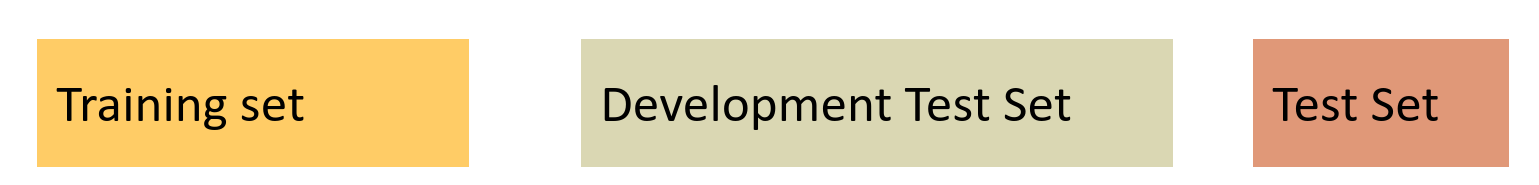
\includegraphics[scale = 0.23]{pics/devsets.png}
\end{figure}

\begin{itemize}
\item \textbf{Training set}: Used to train the model.
\item \textbf{Devset}: Used to tune the model and select the best hyperparameters.
\item \textbf{Testset}: Used to report the final performance of the model.
\end{itemize}


\item This approach ensures that the model is not tuned specifically to the test set, avoiding overfitting.
\item However, it creates a paradox: we want as much data as possible for training, but also for the devset.
\item How do we split the data?

\end{itemize}






\subsection{Cross-validation: Multiple Splits}

\begin{itemize}
\item Cross-validation allows us to use all our data for training and testing without having a fixed training set, devset, and test set.
\item We choose a number $k$ and partition our data into $k$ disjoint subsets called folds.
\item For each iteration, one fold is selected as the test set while the remaining $k-1$ folds are used to train the classifier.
\item We compute the error rate on the test set and repeat this process $k$ times.
\item Finally, we average the error rates from these $k$ runs to obtain an average error rate.
\item 10-fold cross-validation, for example, involves training 10 models on 90\% of the data and testing each model separately.
\item The resulting error rates are averaged to obtain the final performance estimate.
\item However, cross-validation requires the entire corpus to be blind, preventing examination of the data for feature suggestion or understanding system behavior.
\item To address this, a fixed training set and test set are created, and 10-fold cross-validation is performed within the training set.
\item The error rate is computed conventionally in the test set.
\end{itemize}




\begin{center}
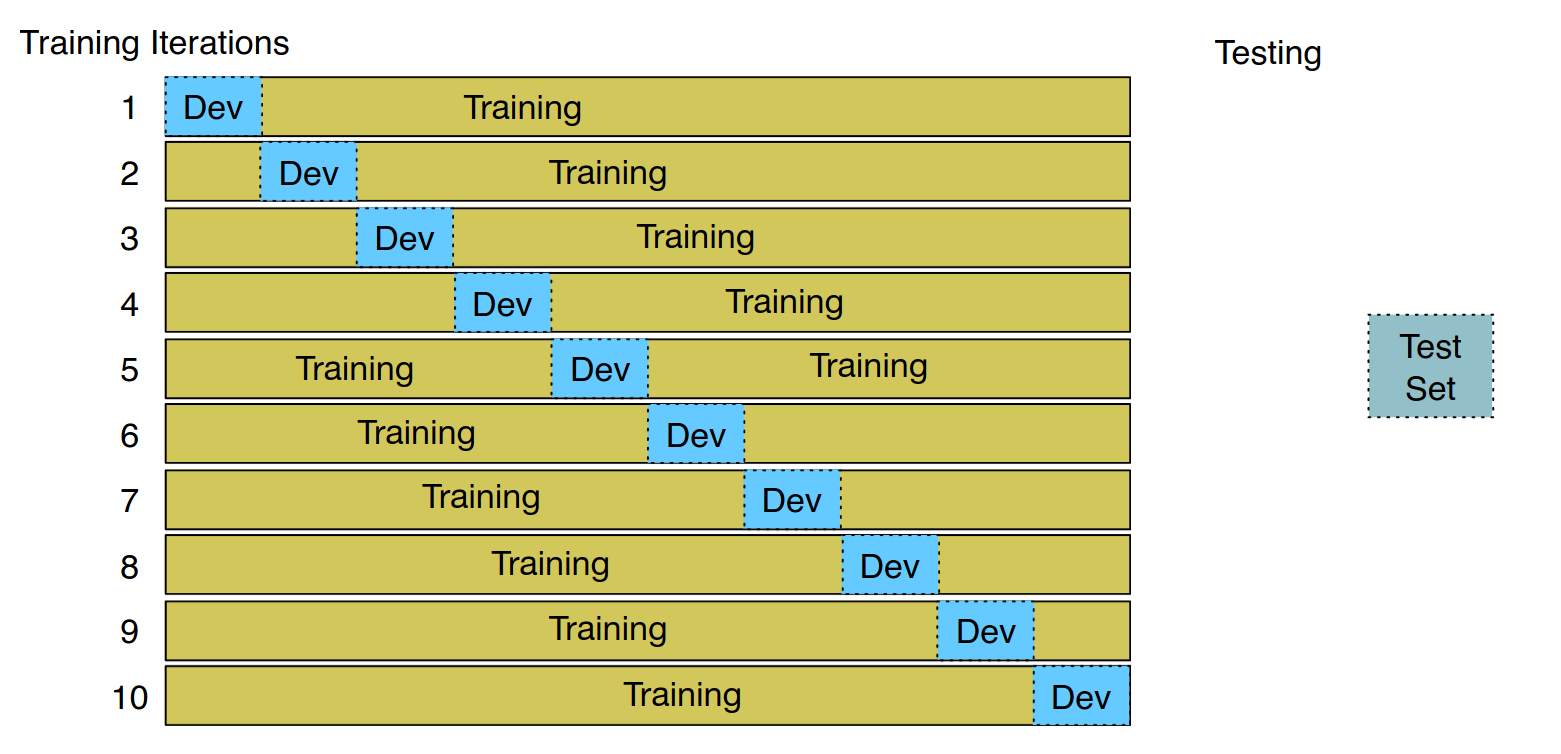
\includegraphics[scale=0.28]{pics/cv.png}
\end{center}




\subsection{Confusion Matrix for 3-class classification}


\begin{center}
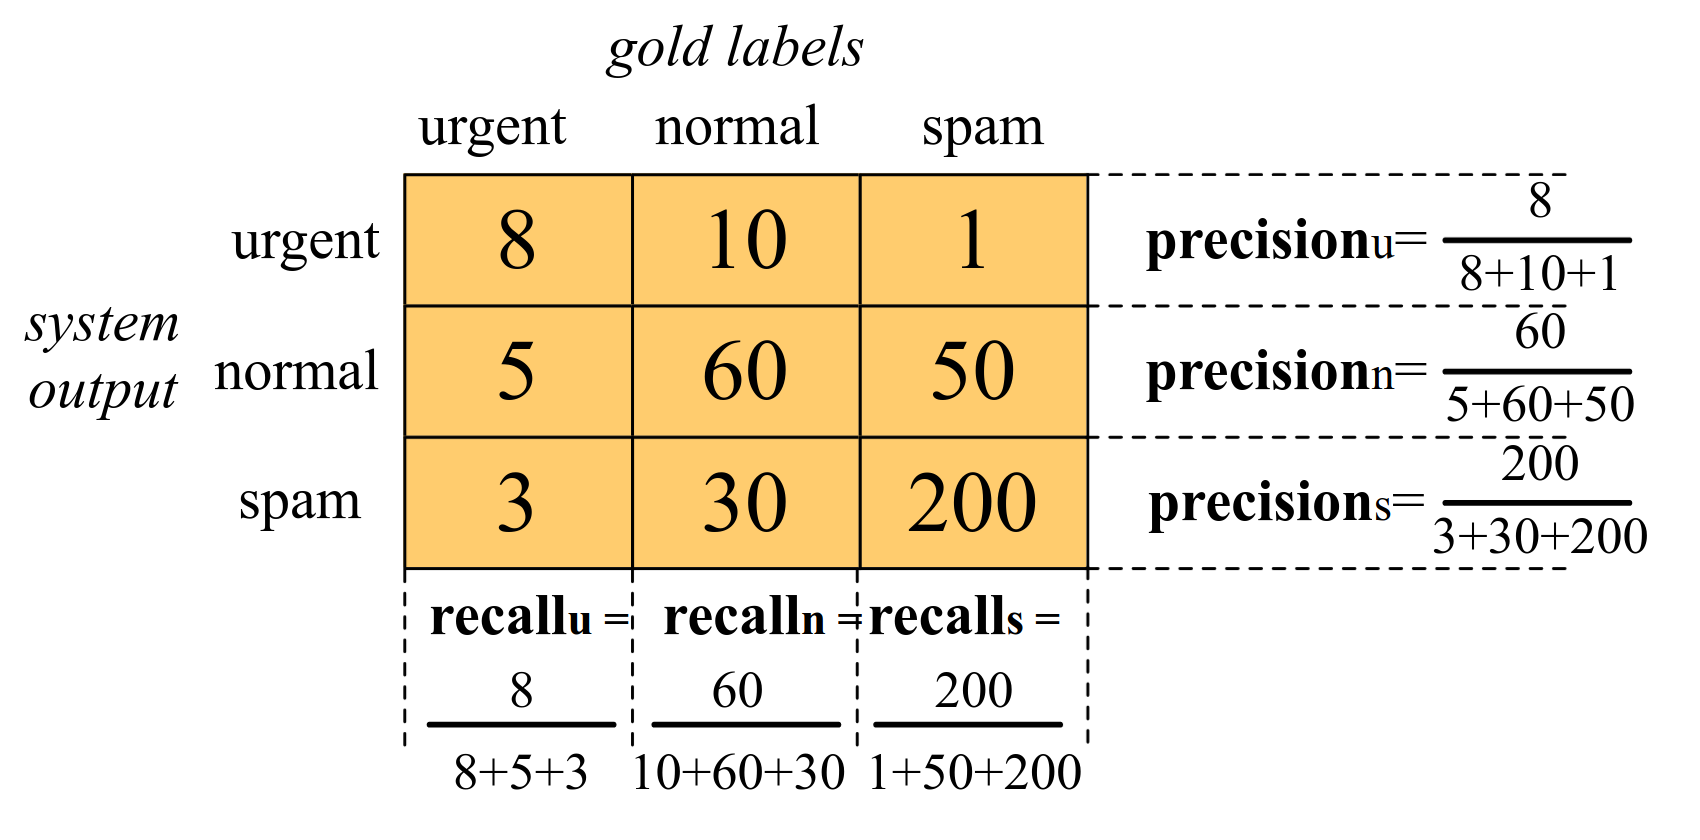
\includegraphics[scale=0.23]{pics/confmatrix.png}
\end{center}


How to combine binary metrics (Precision, Recall, $F_1$) from more than 2 classes to get one metric:
\begin{itemize}
 \item Macroaveraging:
 \begin{itemize}
    \item Compute the performance metrics (Precision, Recall, $F_1$) for each class individually.
    \item Average the metrics over all classes.
 \end{itemize}
 \item Microaveraging:
 \begin{itemize}
    \item Collect the decisions for all classes into one confusion matrix.
    \item Compute Precision and Recall from the confusion matrix.
 \end{itemize}
\end{itemize}



\subsection{Macroaveraging and Microaveraging}


\begin{center}
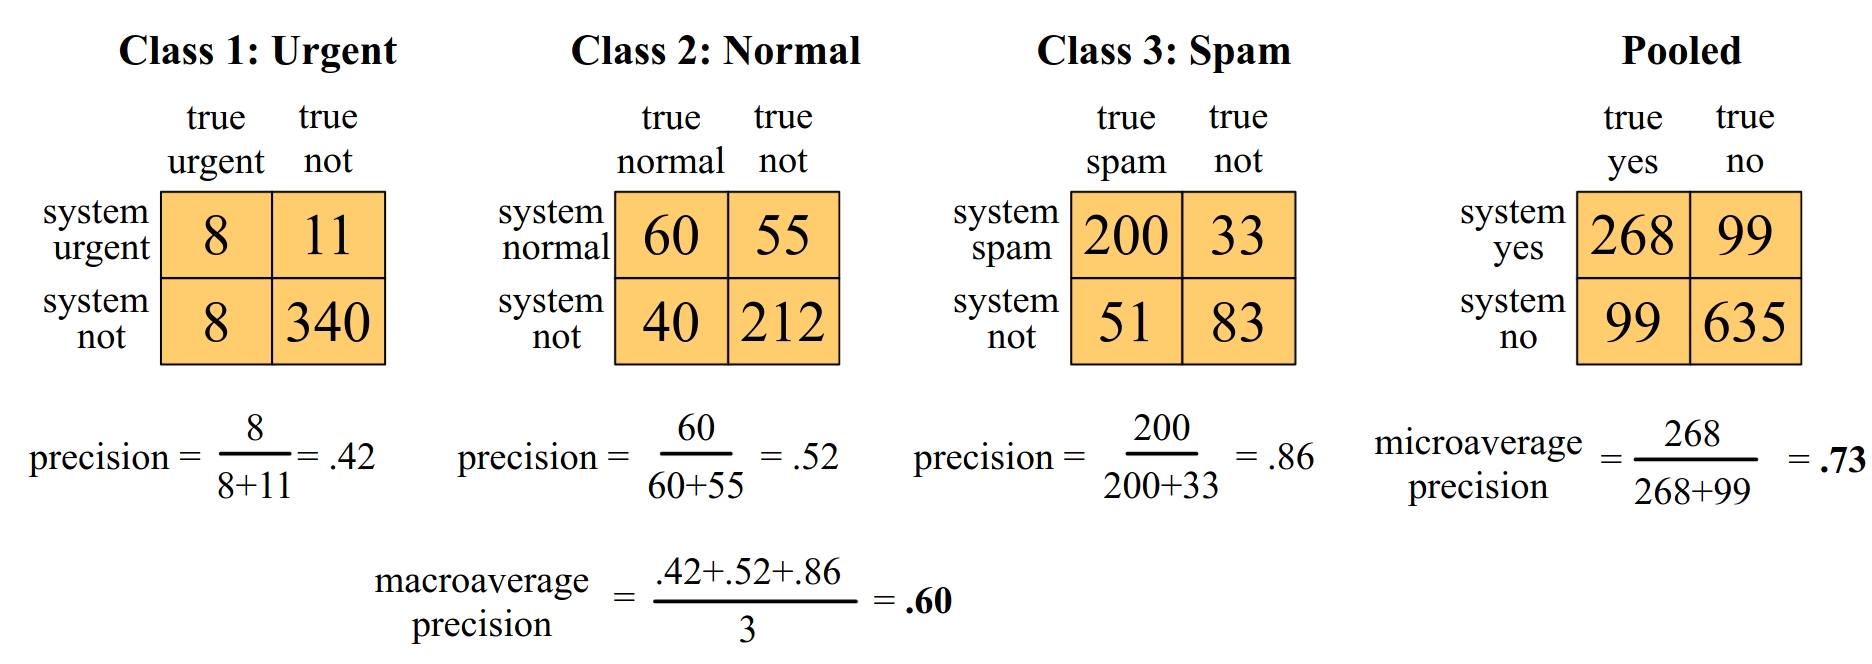
\includegraphics[scale=0.23]{pics/confmatrixmulti.png}
\end{center}
